% ============================================================
%  7.2. COMPRENSIÓN DE LOS DATOS  -- parte del capítulo 7
%  ------------------------------------------------------------
%  Guía 2.7.2: (1) fuentes, (2) variables y diccionario,
%  (3) EDA, (4) distribución, calidad, faltantes, atípicos y
%  relaciones, (5) gráficos y estadísticas, (6) hallazgos que
%  influyen en la preparación y el modelado.
%  Notebook: trufi-data-science/notebooks/01_eda.ipynb
%  Cifras:   resultados/01_eda/metricas.json y CSV de la carpeta.
% ============================================================
\section{Comprensión de los datos}
\label{sec:comprension-datos}

Esta fase examina las tres fuentes del proyecto antes de transformarlas. Tiene tres
propósitos:
\begin{itemize}
  \item medir su calidad;
  \item describir la variable que se va a estimar;
  \item fijar, con evidencia, los criterios que aplicará la preparación de los datos.
\end{itemize}
Se ejecuta en el notebook \var{01_eda}, que lee únicamente \var{data/raw/} y no escribe en
\var{data/}, de modo que ninguna decisión de limpieza se aplica todavía: solo se mide su
efecto. Las cifras de esta sección provienen de \var{resultados/01_eda/metricas.json} y de
los archivos CSV de la misma carpeta.

\subsection{Fuentes de datos}
\label{sec:fuentes-datos}

El proyecto emplea tres fuentes, todas conservadas sin modificar en \var{data/raw/}. La
tabla~\ref{tab:fuentes-datos} resume su origen, su contenido y las condiciones en que se
obtuvieron.

\begin{table}[H]
  \centering
  \caption{Fuentes de datos del proyecto}
  \label{tab:fuentes-datos}
  \interlineadoSimple
  \small
  \begin{tabularx}{\textwidth}{@{}L{0.20\textwidth}L{0.22\textwidth}Y@{}}
    \toprule
    \textbf{Fuente} & \textbf{Productor y obtención} & \textbf{Contenido y cobertura} \\
    \midrule
    Consultas de ``Trufi App'' & Trufi Association; exportaciones semanales del registro de la aplicación, entregadas para este trabajo & 85 archivos CSV que cubren 84 semanas ISO con datos, del 12-09-2022 al 09-06-2024 (la semana del 26-12-2022 al 01-01-2023 viene partida en dos archivos, sin filas repetidas); 1.927.675 consultas con origen, destino, fecha y hora, identificador anónimo de instalación, distancia y municipio de origen y destino \\
    Kontur Population, edición 2023-11-01 & Kontur; conjunto abierto descargado en formato GeoPackage comprimido & Población residente estimada por celda H3 de resolución~8 para toda Bolivia: 145.929 celdas y 12.431.735 habitantes (sección~\ref{subsec:kontur}) \\
    Feed GTFS de Trufi Cochabamba & Trufi Association; generado a partir del mapeo colaborativo en OpenStreetMap & 11 tablas: 43 operadores, 141 líneas y 626 recorridos con su trazado (una línea puede tener varios recorridos, por ejemplo ida y vuelta), 22.320 paradas y frecuencias; vigencia declarada desde el 01-01-2024 \\
    \bottomrule
  \end{tabularx}
  \fuente{Elaboración propia, a partir de \var{01_eda} (secciones 2 y 7) y
  \var{resultados/01_eda/metricas.json}.}
\end{table}

Las tres fuentes cumplen funciones distintas, y conviene fijarlas desde el inicio porque
condicionan todo lo que sigue:
\begin{itemize}
  \item Las \textbf{consultas} producen la variable objetivo, que es el número de consultas
        originadas en cada zona.
  \item \textbf{Kontur} aporta la exposición (la población residente) y las variables de
        entorno poblacional.
  \item El \textbf{GTFS} describe la red mapeada, y en este proyecto se usa solo para
        \emph{interpretar} la brecha, nunca como predictor (sección~\ref{sec:traduccion-necesidad}).
\end{itemize}
Una consulta es una búsqueda de ruta en la aplicación, no un viaje realizado: refleja la
necesidad de información de quienes usan ``Trufi App'', no la movilidad de toda la población
(sección~\ref{subsec:consultas-senal}).

\subsection{Variables y diccionario de datos}
\label{sec:diccionario-datos}

Las exportaciones de consultas llegaron en dos esquemas:
\begin{itemize}
  \item El \emph{lote original} reúne 79 archivos, desde 2022-W37 hasta 2024-W10. Tiene 13
        columnas en codificación UTF-8 y nombres temporales en español (\var{hora},
        \var{dia_de_semana}, \var{dia_de_mes}, \var{fin_de_semana}).
  \item El \emph{lote 2024} reúne 6 archivos, desde 2024-W18 hasta 2024-W23. Tiene 15
        columnas en codificación Latin-1, nombres temporales en inglés y dos campos nuevos
        (\var{year_week_number} y \var{time_of_day}).
\end{itemize}
La consolidación renombra los campos equivalentes a un nombre único y añade tres columnas
de linaje, que registran el archivo, el lote y la codificación de origen de cada fila. Con
ellas, cualquier registro puede rastrearse hasta su archivo. La
tabla~\ref{tab:diccionario-datos} describe las variables resultantes; las marcadas como
\emph{derivadas} no vienen en los archivos, sino que se calculan en la consolidación.

\begin{table}[H]
  \centering
  \caption{Diccionario de datos de las consultas consolidadas}
  \label{tab:diccionario-datos}
  \interlineadoSimple
  \small
  \begin{tabularx}{\textwidth}{@{}L{0.27\textwidth}L{0.13\textwidth}Y@{}}
    \toprule
    \textbf{Variable} & \textbf{Tipo} & \textbf{Significado} \\
    \midrule
    \var{date} & texto & Fecha y hora de la consulta (\texttt{AAAA-MM-DD hh:mm:ss}) \\
    \var{ts} & fecha-hora & Derivada: \var{date} convertida a marca de tiempo \\
    \var{year}, \var{week} & entero & Derivadas: año y semana ISO de \var{ts} \\
    \var{lat_orig}, \var{lon_orig} & real & Coordenadas del origen (WGS84); en el archivo, \var{origin_latitude} y \var{origin_longitude} \\
    \var{lat_dest}, \var{lon_dest} & real & Coordenadas del destino (WGS84) \\
    \var{userID} & texto & Identificador anónimo de la instalación de la aplicación (UUID); no identifica a una persona \\
    \var{distancia} & real & Distancia entre origen y destino; unidad verificada en la sección~\ref{sec:atipicos} (metros) \\
    \var{origin_municipio}, \var{dest_municipio} & texto & Municipio de origen y de destino asignado por la exportación \\
    \var{hour}, \var{day_of_week}, \var{day_of_month}, \var{weekend} & entero & Hora, día de la semana (0 = lunes), día del mes e indicador de fin de semana \\
    \var{year_week_number}, \var{time_of_day} & texto & Semana y franja del día; solo en el lote 2024 \\
    \var{source_file}, \var{source_batch}, \var{source_encoding} & texto & Derivadas: linaje (archivo, lote y codificación de origen) \\
    \bottomrule
  \end{tabularx}
  \fuente{Elaboración propia, a partir de los encabezados de \var{data/raw/*.csv},
  \var{src/lectura.py} y \var{resultados/01_eda/archivos_consultas.csv}.}
\end{table}

De Kontur se usan dos columnas: el identificador de la celda H3 (\var{h3_cell}) y su
población estimada (\var{population}), redondeada a entero. Del GTFS se usan los trazados
(\var{shapes.txt}), a partir de los cuales se calcula la distancia de cada zona a la red
mapeada, y las tablas de líneas, recorridos, paradas y frecuencias para describir la red.
Las variables que se construyen por zona a partir de estas fuentes se documentan en la
sección~\ref{sec:ingenieria-caracteristicas}.

\subsection{Análisis exploratorio de datos}
\label{sec:eda-recorrido}

El análisis exploratorio recorre las fuentes en el orden en que las usará la preparación.
Primero examina la calidad de las consultas, sus valores atípicos y su cobertura en el
tiempo. Después delimita el área de estudio y describe, dentro de ella, la red mapeada y
la población. Por último construye una versión \emph{candidata} de la variable objetivo:
el conteo de consultas por zona, obtenido aplicando en memoria los mismos filtros que
después ejecutará el preprocesamiento.

Trabajar con esa versión candidata tiene una ventaja: las relaciones y la dependencia
espacial se estudian sobre la misma unidad que se modelará, y no sobre consultas
individuales. Las funciones de limpieza que usa este notebook son las mismas que usa el
preprocesamiento (\var{src/limpieza.py}), de modo que las cifras de ambas fases coinciden
por construcción. El notebook termina con tres verificaciones automáticas:
\begin{itemize}
  \item el flujo de filtros cuadra con el total de consultas;
  \item el objetivo suma exactamente las consultas válidas;
  \item no quedan usuarios anómalos ni orígenes fuera del área.
\end{itemize}

\subsection{Calidad, datos faltantes y valores atípicos}
\label{sec:calidad-datos}

\subsubsection{Calidad y consistencia}

La calidad general de las consultas es alta. La tabla~\ref{tab:calidad-consultas} resume
los problemas detectados y su magnitud. En conjunto afectan a 3.097 de 1.927.675
consultas, es decir, al 0,16~\%.

\begin{table}[H]
  \centering
  \caption{Problemas de calidad detectados en las consultas}
  \label{tab:calidad-consultas}
  \interlineadoSimple
  \small
  \begin{tabularx}{\textwidth}{@{}L{0.30\textwidth}rY@{}}
    \toprule
    \textbf{Problema} & \textbf{Consultas} & \textbf{Interpretación} \\
    \midrule
    Origen en (0,0) & 3 & Coordenadas nulas registradas como cero; no localizables \\
    Origen fuera de Bolivia & 9 & Coordenadas imposibles para el servicio \\
    Copia exacta de otra consulta & 60 & Todas las columnas iguales (0,0031~\%); probable duplicación en la exportación \\
    Origen fuera del área de estudio & 2.509 & Consultas aisladas lejos del eje metropolitano (sección~\ref{sec:area-estudio}) \\
    Distancia mayor de 50~km & 283 & Pares origen--destino fuera de la escala urbana (sección~\ref{sec:atipicos}) \\
    Usuario anómalo & 233 & Consultas de dos instalaciones con uso no humano (sección~\ref{sec:atipicos}) \\
    \bottomrule
  \end{tabularx}
  \fuente{Elaboración propia, a partir de \var{resultados/01_eda/flujo_candidato.csv},
  \var{duplicados.csv} y \var{metricas.json}. Las cifras corresponden a la aplicación
  secuencial de los filtros; una consulta se cuenta en el primer filtro que la excluye.}
\end{table}

Los duplicados se examinaron con cuatro definiciones de creciente laxitud. Las copias
exactas y las que repiten origen, destino y marca de tiempo coinciden (60 en ambos casos).
Si se exige solo el mismo usuario y el mismo instante, aparecen 90. Como las 30 adicionales
difieren en el origen o el destino, pueden ser búsquedas legítimas distintas. Por eso solo
se considera duplicado lo que es idéntico en todas las columnas.

\subsubsection{Datos faltantes}
\label{sec:datos-faltantes-eda}

Ninguna de las columnas que usa el proyecto tiene valores nulos: coordenadas,
identificador, fecha y distancia están completas en ambos lotes. Las dos únicas columnas
con nulos, \var{year_week_number} y \var{time_of_day}, aparecen vacías en el 91,6~\% de
las filas. No es un faltante aleatorio, sino \emph{estructural}: esas columnas no existen en
el lote original. Como ambas pueden recalcularse a partir de la fecha, no se usan.

La ausencia de datos relevante para el proyecto está en otro nivel: faltan semanas enteras
de registro (sección~\ref{sec:cobertura-temporal}) y hay zonas pobladas sin ninguna
consulta (sección~\ref{sec:distribucion-objetivo}). Ninguna de las dos se imputa, en
coherencia con el alcance (capítulo~\ref{cap:alcance}) y con el tratamiento de datos
faltantes expuesto en la sección~\ref{subsec:datos-faltantes}. El hueco temporal se
documenta y se neutraliza al expresar lo esperado por semana observada. En cuanto a los
ceros, una zona poblada sin consultas es información, no ausencia de dato.

\subsubsection{Valores atípicos: distancia y usuarios anómalos}
\label{sec:atipicos}

\textbf{Distancia.} El campo \var{distancia} no traía unidad declarada. Para verificarla,
se comparó con la distancia geodésica entre origen y destino calculada de forma
independiente, en una muestra de 200.000 consultas. El error relativo mediano fue del
0,142~\%, lo que confirma que el campo está en metros y corresponde a la distancia en
línea recta.

La distribución (figura~\ref{fig:distancia}) muestra el comportamiento esperado de un
servicio urbano:
\begin{itemize}
  \item la mediana es de 3,39~km;
  \item el 90~\% de las consultas no supera los 10,26~km;
  \item el percentil 99,9 llega a 40,7~km.
\end{itemize}
Por encima de 50~km aparece una cola dispersa (el 0,04~\% de las consultas) que llega a
miles de kilómetros y que no corresponde a viajes posibles en la red urbana.

\begin{figure}[H]
  \centering
  \caption{Distribución de la distancia origen--destino de las consultas}
  \label{fig:distancia}
  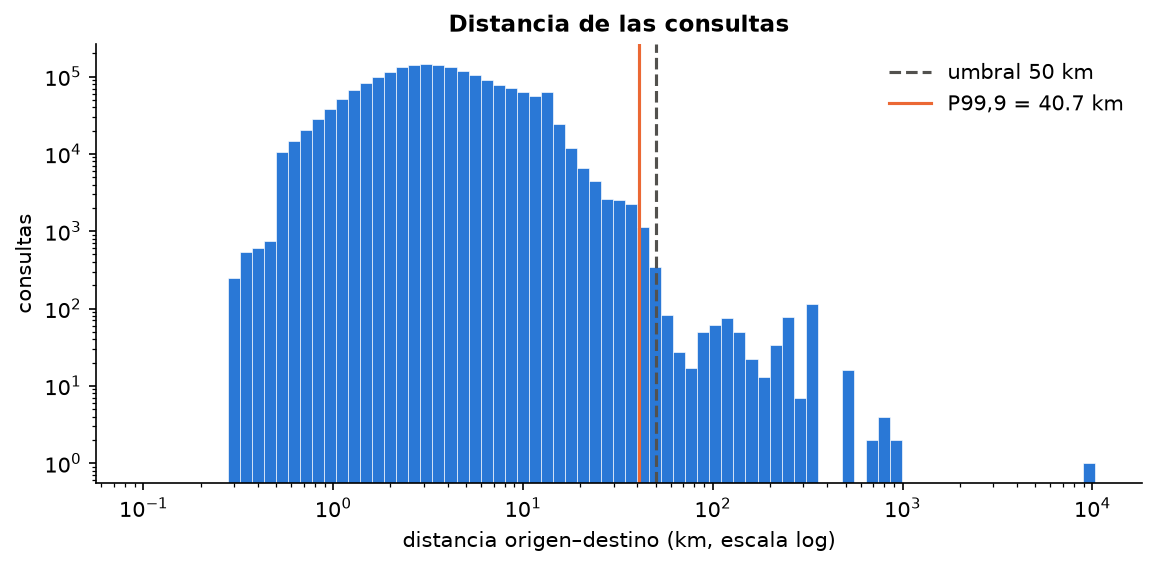
\includegraphics[width=0.75\textwidth]{imagenes/07_desarrollo/7_2_comprension_datos/distancia.png}
  \fuente{Elaboración propia, a partir de \var{01_eda} (sección 3). Ambos ejes en escala
  logarítmica; la línea discontinua marca el umbral de 50~km.}
\end{figure}

El umbral de 50~km se aplica a las \emph{consultas} y no a la delimitación del área. Una
consulta con destino lejano puede tener un origen perfectamente válido dentro de la
ciudad. Si el área se recortara con ese criterio, zonas reales quedarían fuera.

\textbf{Usuarios anómalos.} Hay 130.545 identificadores de instalación distintos. Para
detectar un uso no humano, por ejemplo pruebas automatizadas o extracción masiva de
rutas, se definieron seis señales por usuario, con umbrales fijados en \var{config.py}:
\begin{itemize}
  \item más de 1.000 consultas en total (volumen);
  \item más de 50 consultas por día activo (intensidad);
  \item más de 200 zonas de origen distintas (dispersión);
  \item más de 100 consultas en un mismo día (ráfaga);
  \item menos del 5~\% de pares origen--destino repetidos entre usuarios con más de 100
        consultas (sin rutina);
  \item un intervalo mediano menor de 60~segundos entre consultas consecutivas (rapidez).
\end{itemize}

La tabla~\ref{tab:senales-usuario} muestra cuántos usuarios activan cada señal y justifica
que se exijan al menos dos. La señal de rapidez, por sí sola, marcaría a 10.511
instalaciones. Esas instalaciones corresponden a un comportamiento humano habitual:
repetir una búsqueda o corregir el destino en pocos segundos. Exigir dos señales
simultáneas deja solo dos instalaciones anómalas, con 233 consultas en total.

\begin{table}[H]
  \centering
  \caption{Usuarios que activan cada señal de uso anómalo}
  \label{tab:senales-usuario}
  \interlineadoSimple
  \small
  \begin{tabular}{@{}lr@{}}
    \toprule
    \textbf{Señal} & \textbf{Usuarios} \\
    \midrule
    Volumen ($>$ 1.000 consultas) & 1 \\
    Intensidad ($>$ 50 consultas por día activo) & 1 \\
    Dispersión ($>$ 200 zonas de origen) & 0 \\
    Ráfaga ($>$ 100 consultas en un día) & 1 \\
    Sin rutina ($<$ 5~\% de pares repetidos) & 0 \\
    Rapidez (intervalo mediano $<$ 60~s) & 10.511 \\
    \midrule
    \textbf{Marcados como anómalos ($\geq$ 2 señales)} & \textbf{2} \\
    \bottomrule
  \end{tabular}
  \fuente{Elaboración propia, a partir de \var{resultados/01_eda/usuarios_senales.csv} y
  \var{src/limpieza.py}.}
\end{table}

\subsection{Distribución temporal y espacial}
\label{sec:distribucion-datos}

\subsubsection{Cobertura temporal}
\label{sec:cobertura-temporal}

El período declarado va del 12 de septiembre de 2022 al 9 de junio de 2024, es decir,
91 semanas ISO. Hay datos en 84 de ellas, repartidos en 85 archivos: la semana que va del
26 de diciembre de 2022 al 1 de enero de 2023 se exportó en dos archivos, uno con los días
26 a 31 de diciembre (11.622 consultas) y otro con el 1 de enero (695), sin filas repetidas
entre ambos. De las 84 semanas, 78 tienen registros los siete días. Faltan
siete semanas consecutivas, del 11 de marzo al 28 de abril de 2024, sin ninguna consulta
(figura~\ref{fig:cobertura-semanal}).

\begin{figure}[H]
  \centering
  \caption{Consultas por semana y hueco sin datos de 2024}
  \label{fig:cobertura-semanal}
  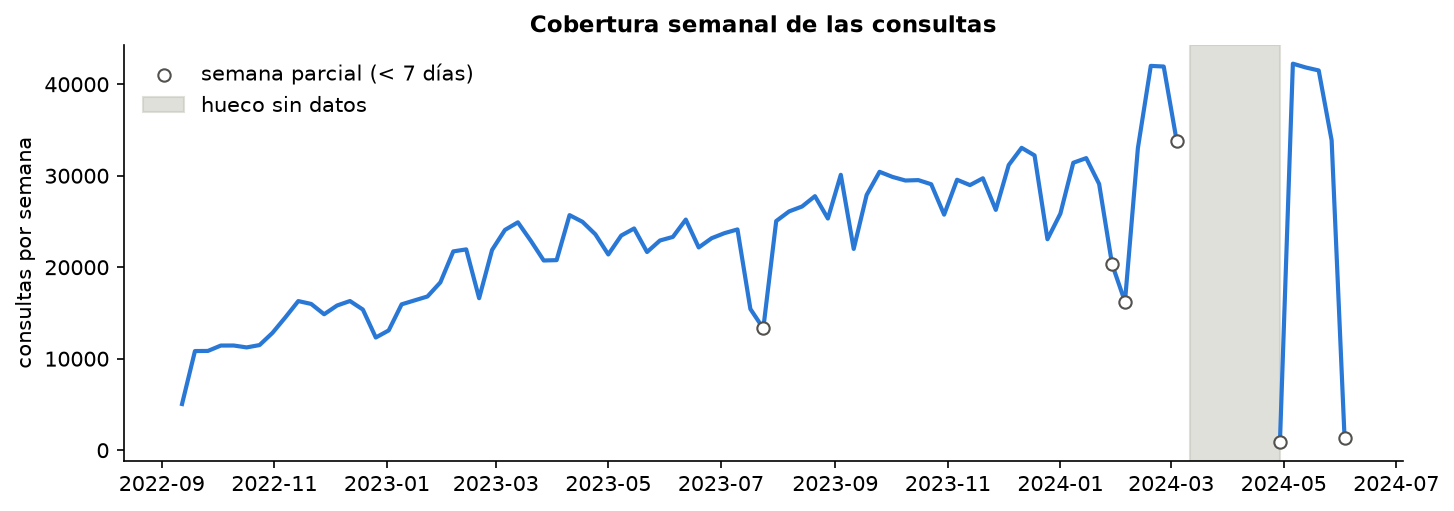
\includegraphics[width=\textwidth]{imagenes/07_desarrollo/7_2_comprension_datos/cobertura_semanal.png}
  \fuente{Elaboración propia, a partir de \var{01_eda} (sección 5). Los círculos marcan
  semanas parciales (menos de siete días con datos).}
\end{figure}

La serie muestra un crecimiento sostenido del uso: de unas 11.000 consultas semanales a
fines de 2022 a más de 30.000 a fines de 2023. La media semanal pasa de 22.731 consultas
antes del hueco a 39.864 después. El hueco coincide exactamente con el cambio de esquema:
el lote 2024, con dos columnas nuevas y otra codificación, empieza en la primera semana
posterior. Esa coincidencia sugiere una interrupción del proceso de exportación, y no una
caída real del uso.

El conjunto de datos disponible corresponde a las exportaciones que Trufi Association pudo
extraer y entregar en el plazo del proyecto; el resto del registro continúa en proceso de
exportación. El hueco de siete semanas y el cambio de esquema son consistentes con esa
interrupción, aunque la causa exacta no pudo confirmarse. Esta limitación se retoma en la
sección~\ref{sec:limitaciones} y en la recomendación R8. El registro es, por tanto,
parcial y puede ampliarse, y los resultados describen los datos entregados.

El hueco no afecta a la unidad de análisis, que es el total de consultas por zona
acumulado en todo el período. Sí afecta a la lectura de ese total como volumen semanal.
Por eso la preparación calcula las semanas equivalentes realmente observadas
(sección~\ref{sec:transformaciones}), y la evaluación comprueba si la lista de zonas
cambia al usar solo el período anterior al hueco (sección~\ref{sec:interpretacion-resultados}).

El perfil horario y semanal (figura~\ref{fig:perfil-temporal}) confirma que el registro
refleja un uso cotidiano de transporte:
\begin{itemize}
  \item la actividad crece desde las 6~h y alcanza su máximo a las 14~h, con el 8,2~\% de
        las consultas;
  \item los días laborables reúnen entre el 14~\% y el 17~\% de las consultas cada uno;
  \item el fin de semana concentra el 22,8~\%, y el domingo es el día de menor uso.
\end{itemize}
Este perfil no se modela, porque el alcance excluye la dimensión temporal. Se incluye como
evidencia de que las consultas corresponden a necesidades reales de desplazamiento y no a
tráfico artificial.

\begin{figure}[H]
  \centering
  \caption{Distribución de las consultas por hora del día y por día de la semana}
  \label{fig:perfil-temporal}
  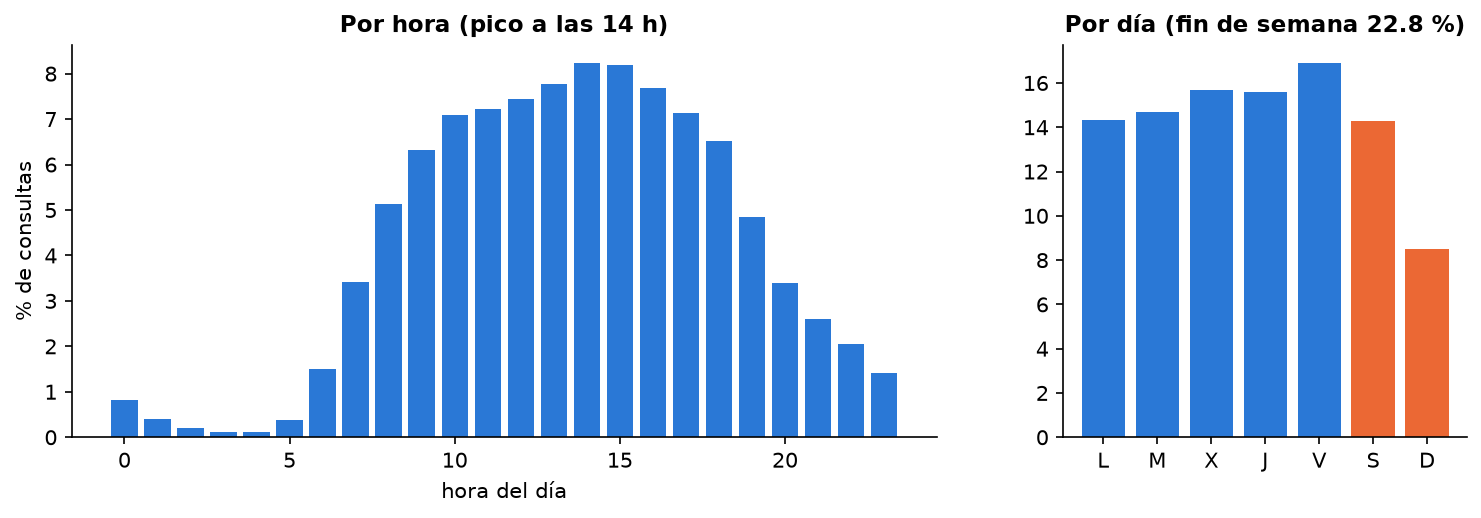
\includegraphics[width=\textwidth]{imagenes/07_desarrollo/7_2_comprension_datos/perfil_temporal.png}
  \fuente{Elaboración propia, a partir de \var{01_eda} (sección 5) y
  \var{resultados/01_eda/perfil_temporal.csv}.}
\end{figure}

\subsubsection{Distribución espacial y área de estudio}
\label{sec:area-estudio}

El alcance dejó abierta la delimitación operativa del entorno del eje metropolitano
(capítulo~\ref{cap:alcance}), y esta fase la fija a partir de los propios datos. El primer
intento fue la envolvente de todas las zonas H3 con al menos un origen válido, que
abarcaría 485.940,1~km\textsuperscript{2}, más de un tercio de la superficie de Bolivia.
El motivo es que unas pocas consultas aisladas, muy alejadas, estiran el contorno. Ese
resultado muestra que un área definida por los datos crudos es frágil ante atípicos
geográficos.

La solución adoptada identifica la \emph{componente contigua principal} de las zonas H3
con orígenes válidos. Esa componente es el mayor conjunto de zonas conectadas entre sí por
vecindad directa. El área es su envolvente, ampliada con un margen de 1~km. La
tabla~\ref{tab:variantes-area} compara esta opción con otras más laxas, en las que dos
zonas se consideran conectadas aunque estén separadas por uno o dos anillos vacíos.

\begin{table}[H]
  \centering
  \caption{Variantes de delimitación del área de estudio}
  \label{tab:variantes-area}
  \interlineadoSimple
  \small
  \begin{tabular}{@{}lrr@{}}
    \toprule
    \textbf{Variante} & \textbf{Zonas H3} & \textbf{Área (km\textsuperscript{2})} \\
    \midrule
    Todas las zonas con orígenes válidos & 1.516 & 485.940,1 \\
    \textbf{Componente contigua, vecindad directa ($k=1$)} & \textbf{919} & \textbf{1.505,7} \\
    Componente con separación de hasta un anillo ($k=2$) & 1.076 & 1.965,4 \\
    Componente con separación de hasta dos anillos ($k=3$) & 1.195 & 3.040,9 \\
    \bottomrule
  \end{tabular}
  \fuente{Elaboración propia, a partir de \var{resultados/01_eda/area_variantes.csv}. El área
  incluye el margen de 1~km.}
\end{table}

La variante elegida mide 1.505,7~km\textsuperscript{2} y contiene el 99,87~\% de los
orígenes válidos (figura~\ref{fig:area-estudio}). Las variantes más laxas duplican el área
para ganar una fracción mínima de consultas, a costa de incorporar zonas rurales casi sin
uso. Las 2.509 consultas que quedan fuera son las que la
tabla~\ref{tab:calidad-consultas} registra como ``origen fuera del área de estudio''.

\begin{figure}[H]
  \centering
  \caption{Orígenes de las consultas y área de estudio delimitada}
  \label{fig:area-estudio}
  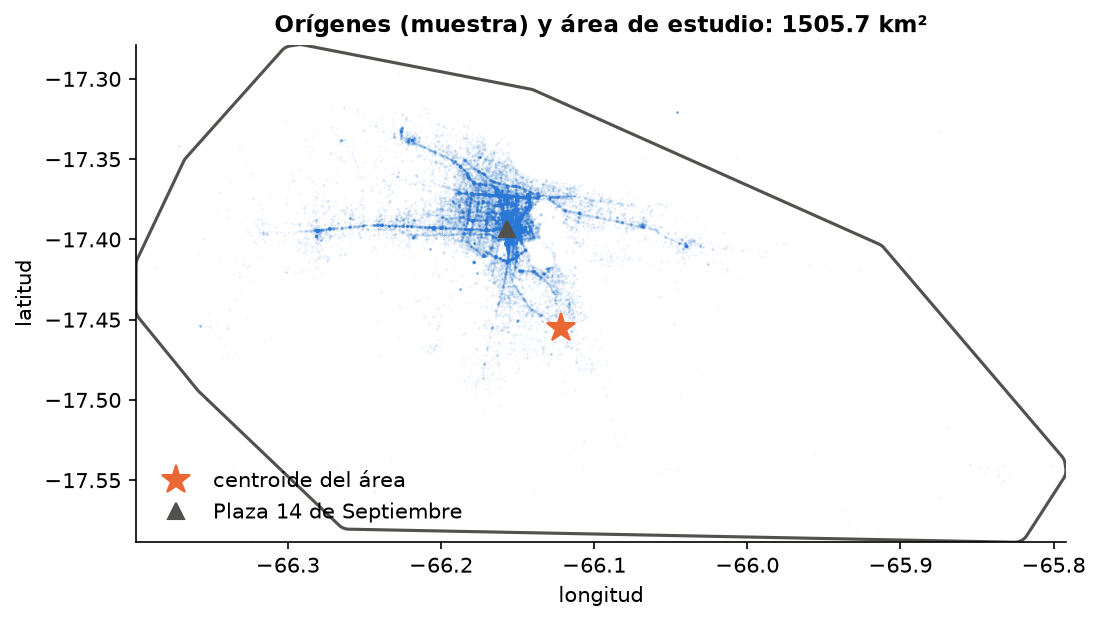
\includegraphics[width=0.85\textwidth]{imagenes/07_desarrollo/7_2_comprension_datos/area_estudio.png}
  \fuente{Elaboración propia, a partir de \var{01_eda} (sección 6). Puntos: muestra de
  orígenes; contorno: área de estudio; triángulo: Plaza 14 de Septiembre; estrella:
  centroide geométrico del área.}
\end{figure}

La figura revela además un hecho que se retoma en la preparación: el centroide geométrico
del área está a 7,82~km de la Plaza 14 de Septiembre, fuera del núcleo donde se concentran
los orígenes. Un ``centro'' calculado a partir de la forma del área no representa el
centro de actividad de la ciudad.

Dentro del área se localizan 1.577 celdas de Kontur (por la posición de su centroide), con
1.223.871 habitantes. De ellas, 609 no registran ningún origen de consulta en los datos
sin depurar; tras la limpieza son 611, porque dos celdas solo tenían consultas que la limpieza
excluyó (sección~\ref{sec:limpieza}). Además, 202 tienen
menos de 10 habitantes. La red mapeada cubre la mayor parte del territorio con demanda
(figura~\ref{fig:gtfs-red}): el 99,47~\% de los orígenes está a 500~m o menos de algún
trazado GTFS. Los trazados tienen una longitud mediana de 20,22~km y suman
12.737,3~km. La frecuencia mediana declarada es de un servicio cada 5~minutos.

\begin{figure}[H]
  \centering
  \caption{Trazados de la red mapeada (GTFS) y orígenes de las consultas}
  \label{fig:gtfs-red}
  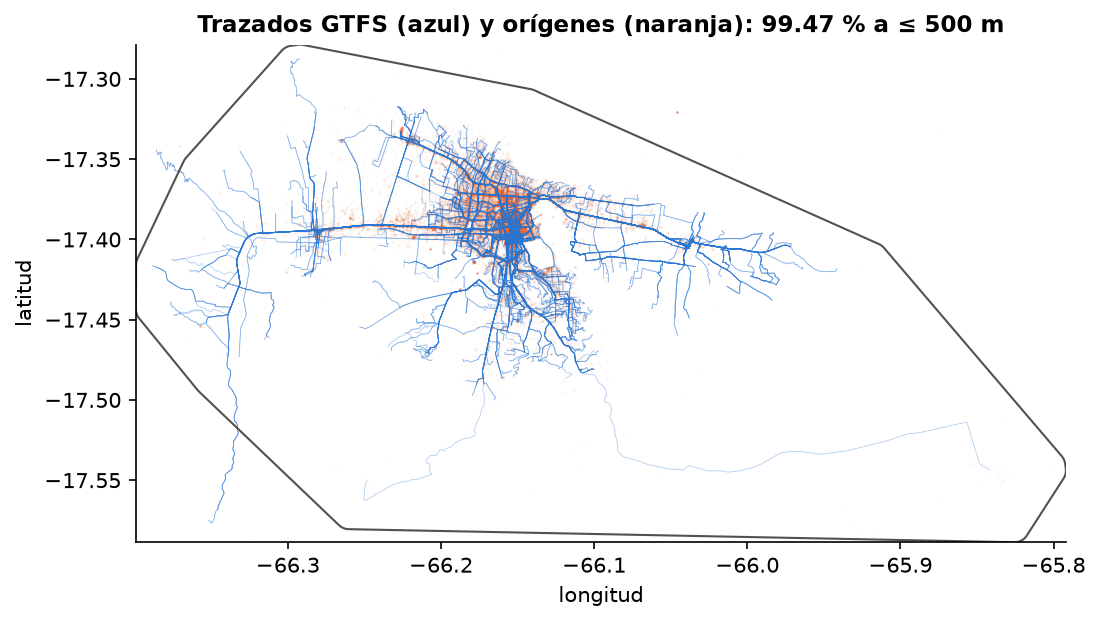
\includegraphics[width=0.85\textwidth]{imagenes/07_desarrollo/7_2_comprension_datos/gtfs_red_y_demanda.png}
  \fuente{Elaboración propia, a partir de \var{01_eda} (sección 7). Azul: trazados de
  \var{shapes.txt}; naranja: orígenes.}
\end{figure}

Que casi todos los orígenes estén cerca de un trazado no implica que la red esté completa.
Las consultas nacen donde la aplicación ya es útil: una zona sin rutas mapeadas genera
pocas consultas precisamente porque la aplicación no le ofrece respuestas. Este sesgo de
selección es la razón por la que la cobertura no puede usarse para estimar lo esperado
(sección~\ref{sec:traduccion-necesidad}). También hay que tener en cuenta que el feed
declara una vigencia posterior a buena parte del período de consultas, una limitación ya
reconocida en el capítulo~\ref{cap:alcance}.

\subsubsection{Distribución de la variable objetivo}
\label{sec:distribucion-objetivo}

La variable objetivo candidata, \var{query_count}, es el número de consultas válidas
originadas en cada zona H3 de resolución~8 durante el período. Dentro del área hay 1.628
zonas. Para que una tasa por habitante sea estable, se exige un mínimo de 10 habitantes;
1.381 zonas lo cumplen. La figura~\ref{fig:objetivo-distribucion} resume la distribución
del conteo en esas 1.381 zonas.

\begin{figure}[H]
  \centering
  \caption{Distribución del conteo de consultas por zona y curva de Lorenz}
  \label{fig:objetivo-distribucion}
  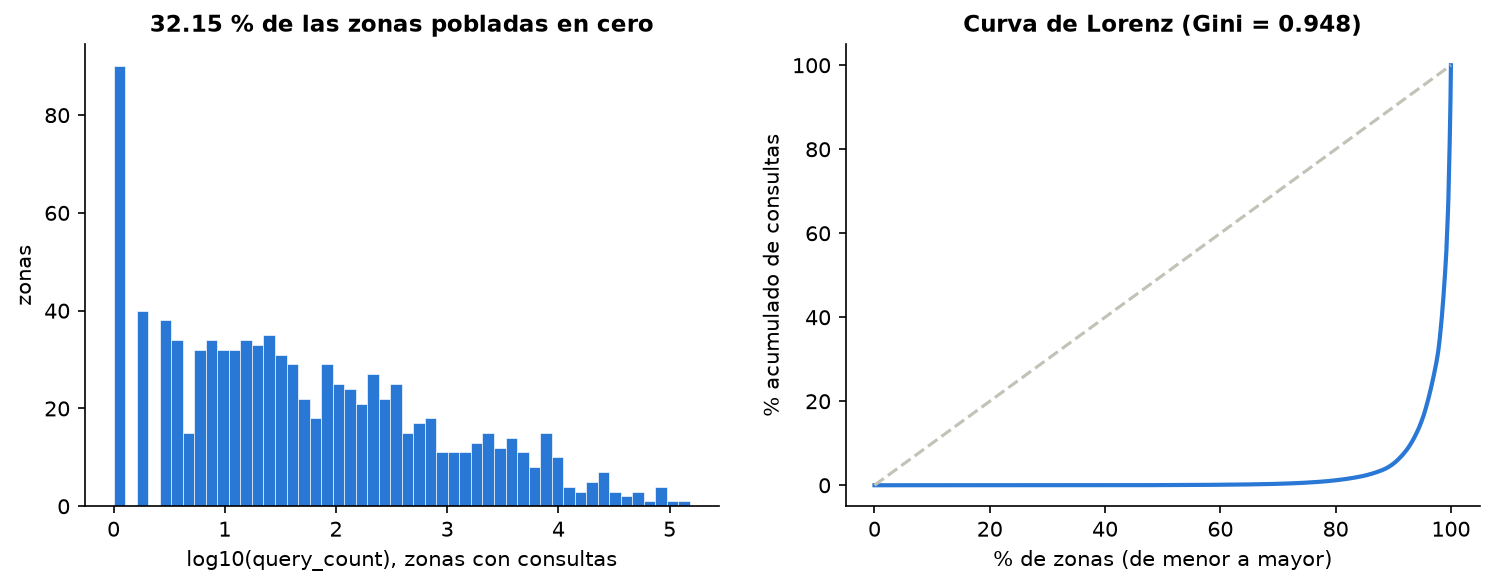
\includegraphics[width=\textwidth]{imagenes/07_desarrollo/7_2_comprension_datos/objetivo_distribucion.png}
  \fuente{Elaboración propia, a partir de \var{01_eda} (sección 9). Izquierda: histograma de
  $\log_{10}$ del conteo en las zonas con consultas; derecha: proporción acumulada de
  consultas frente a proporción acumulada de zonas.}
\end{figure}

Tres rasgos caracterizan la distribución y condicionan el modelado:
\begin{itemize}
  \item \textbf{Abundancia de ceros.} El 32,15~\% de las zonas pobladas (444 de 1.381) no
        registra ninguna consulta. Esos ceros se conservan: son justamente el tipo de zona
        que el problema busca examinar (capítulo~\ref{cap:problema}).
  \item \textbf{Concentración extrema.} El coeficiente de Gini es de 0,948, y las diez
        zonas con más consultas reúnen el 42~\% del total. Como muestra la curva de Lorenz,
        el 80~\% de las zonas aporta menos del 5~\% de las consultas.
  \item \textbf{Sobredispersión.} La varianza del conteo es 46.569 veces su media. Un modelo
        de Poisson supone varianza igual a la media
        (sección~\ref{subsec:datos-conteo}), así que este resultado anticipa que ese
        supuesto no se cumplirá y justifica incluir alternativas que lo relajen.
\end{itemize}

\subsection{Relaciones entre variables y dependencia espacial}
\label{sec:relaciones-variables}

Para examinar qué información territorial se asocia con las consultas, se calculó la
correlación de Spearman entre el conteo por zona y cada variable candidata. La correlación
de Spearman se basa en rangos, por lo que es robusta a la asimetría de los datos. Se
calculó también frente a la \emph{tasa} de consultas por 1.000 habitantes, para distinguir
la asociación que se debe solo al tamaño de la población de la que se debe al contexto. La
tabla~\ref{tab:relaciones} presenta los resultados.

\begin{table}[H]
  \centering
  \caption{Correlación de Spearman de las variables candidatas con el conteo y con la tasa}
  \label{tab:relaciones}
  \interlineadoSimple
  \small
  \begin{tabularx}{\textwidth}{@{}L{0.22\textwidth}Yrr@{}}
    \toprule
    \textbf{Variable} & \textbf{Significado} & \textbf{Conteo} & \textbf{Tasa} \\
    \midrule
    \var{population} & Habitantes de la zona (Kontur) & 0,855 & 0,710 \\
    \var{pop_ring1} & Habitantes del primer anillo de seis zonas vecinas & 0,836 & 0,721 \\
    \var{pop_ring2} & Habitantes del segundo anillo de vecinas & 0,804 & 0,701 \\
    \var{dist_centro_km} & Distancia a la Plaza 14 de Septiembre (km) & $-0{,}697$ & $-0{,}677$ \\
    \var{dist_centroide_km} & Distancia al centroide geométrico del área (km) & $-0{,}476$ & $-0{,}485$ \\
    \var{dist_trazado_m} & Distancia al trazado GTFS más cercano (m); solo contraste & $-0{,}763$ & $-0{,}701$ \\
    \bottomrule
  \end{tabularx}
  \fuente{Elaboración propia, a partir de \var{resultados/01_eda/relaciones.csv}; 1.381 zonas
  con al menos 10 habitantes.}
\end{table}

De la tabla se desprenden tres lecturas:
\begin{itemize}
  \item La población es la variable más asociada con el conteo, lo que justifica tratarla
        como exposición. Las variables de entorno siguen asociadas con la \emph{tasa}
        (0,72 para la población vecina y $-0{,}68$ para la distancia al centro), de modo que
        el contexto aporta información más allá del tamaño de la zona.
  \item La distancia a la Plaza se asocia bastante más que la distancia al centroide del
        área ($-0{,}697$ frente a $-0{,}476$), lo que confirma que el centro de referencia
        debe fijarse de forma externa a los datos y no derivarse de la forma del área.
  \item La distancia al trazado GTFS tiene una asociación fuerte, pero se reserva para el
        contraste por el sesgo de selección descrito en la sección~\ref{sec:area-estudio}.
\end{itemize}

La figura~\ref{fig:objetivo-poblacion} muestra la relación con la población en escala
logarítmica. La asociación es clara, pero la dispersión es enorme: zonas con población
similar difieren en varios órdenes de magnitud. Las zonas alejadas del trazado (en
naranja) se concentran en la parte baja.

\begin{figure}[H]
  \centering
  \caption{Consultas por zona frente a su población, según la distancia al trazado}
  \label{fig:objetivo-poblacion}
  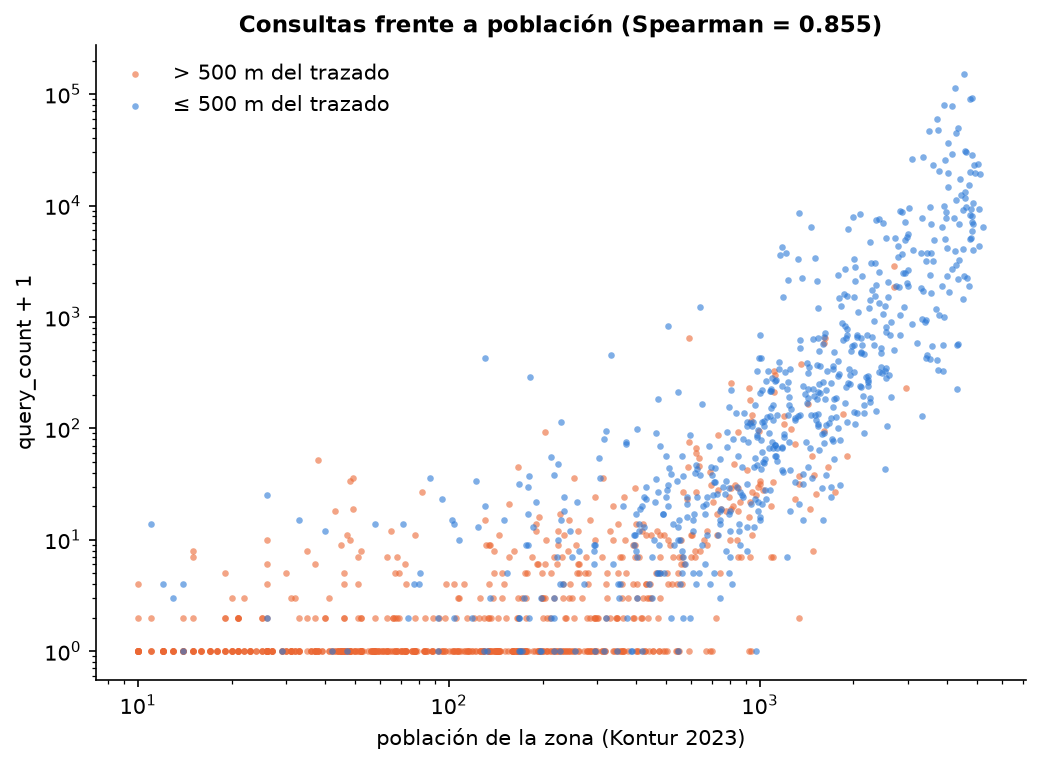
\includegraphics[width=0.75\textwidth]{imagenes/07_desarrollo/7_2_comprension_datos/objetivo_vs_poblacion.png}
  \fuente{Elaboración propia, a partir de \var{01_eda} (sección 10). Ambos ejes en escala
  logarítmica; al conteo se le suma 1 para representar los ceros.}
\end{figure}

\textbf{Dependencia espacial.} Se midió con el índice $I$ de Moran de la tasa de consultas
(sección~\ref{subsec:autocorrelacion}), tomando como vecinas las zonas situadas a $k$
anillos H3 de distancia, con $k$ de 1 a 5. La significación se evaluó con 499
permutaciones, por lo que el menor $p$-valor alcanzable es 0,002.

\begin{table}[H]
  \centering
  \caption{Correlograma del índice de Moran de la tasa de consultas}
  \label{tab:correlograma}
  \interlineadoSimple
  \small
  \begin{tabular}{@{}crrr@{}}
    \toprule
    \textbf{\celda{Orden de\\vecindad $k$}} & \textbf{\celda{Distancia\\aproximada (km)}} & \textbf{$I$ de Moran} & \textbf{$p$-valor} \\
    \midrule
    1 & 0,92 & 0,7161 & 0,002 \\
    2 & 1,84 & 0,6399 & 0,002 \\
    3 & 2,76 & 0,5773 & 0,002 \\
    4 & 3,68 & 0,5094 & 0,002 \\
    5 & 4,60 & 0,4603 & 0,002 \\
    \bottomrule
  \end{tabular}
  \fuente{Elaboración propia, a partir de \var{resultados/01_eda/autocorrelacion.csv}.}
\end{table}

El correlograma (tabla~\ref{tab:correlograma}) muestra una autocorrelación positiva muy
fuerte entre vecinas inmediatas ($I = 0{,}72$), que decae lentamente y sigue en 0,46 a
unos 4,6~km. El indicador local LISA (figura~\ref{fig:lisa}) localiza esa estructura:
\begin{itemize}
  \item un gran núcleo de 295 zonas \emph{alto-alto} (tasa alta rodeada de tasas altas) en
        el centro y los ejes de Cercado y Sacaba;
  \item 253 zonas \emph{bajo-bajo} en la periferia y en el sur del valle;
  \item pocos casos discordantes (41 alto-bajo y 3 bajo-alto).
\end{itemize}

\begin{figure}[H]
  \centering
  \caption{Agrupamientos locales de la tasa de consultas (LISA)}
  \label{fig:lisa}
  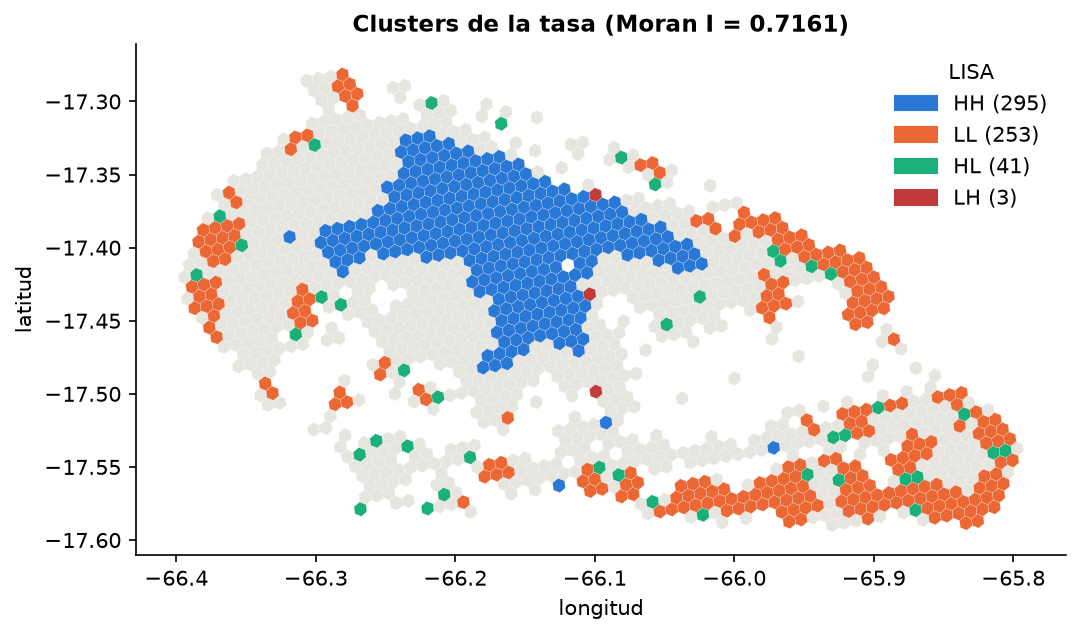
\includegraphics[width=0.85\textwidth]{imagenes/07_desarrollo/7_2_comprension_datos/lisa.png}
  \fuente{Elaboración propia, a partir de \var{01_eda} (sección 11). HH: alto-alto;
  LL: bajo-bajo; HL: alto-bajo; LH: bajo-alto; gris: sin agrupamiento significativo.}
\end{figure}

Este hallazgo tiene dos consecuencias metodológicas directas:
\begin{itemize}
  \item Las zonas vecinas se parecen, de modo que una partición aleatoria en entrenamiento
        y prueba colocaría a cada zona de prueba junto a vecinas casi idénticas y
        sobreestimaría el desempeño. La validación y la reserva de prueba deben hacerse por
        \emph{bloques} espaciales de varios kilómetros (sección~\ref{subsec:validacion-espacial}).
  \item La tasa de las zonas vecinas contiene información útil para estimar la de una zona,
        lo que motiva incluir entre las técnicas un estimador de vecindad
        (sección~\ref{sec:seleccion-algoritmos}).
\end{itemize}

\subsection{Estadísticas descriptivas del conjunto de datos H3}
\label{sec:estadisticas-descriptivas}

La tabla~\ref{tab:descriptivos} reúne las estadísticas de las variables numéricas por zona
que se usan en las fases siguientes. Se calculan sobre las 1.381 zonas que entrarán al
modelo.

\begin{table}[H]
  \centering
  \caption{Estadísticas descriptivas de las variables por zona}
  \label{tab:descriptivos}
  \interlineadoSimple
  \small
  \begin{tabular}{@{}lrrrrrrr@{}}
    \toprule
    \textbf{Variable} & \textbf{Media} & \textbf{Desv. est.} & \textbf{Mín.} & \textbf{P25} & \textbf{Mediana} & \textbf{P75} & \textbf{Máx.} \\
    \midrule
    \var{query_count} (consultas) & 1.393,4 & 8.058,4 & 0 & 0 & 6 & 109 & 152.494 \\
    \var{population} (hab.) & 887,5 & 1.162,6 & 10 & 97 & 388 & 1.183 & 5.240 \\
    \var{pop_ring1} (hab.) & 5.221,8 & 6.363,6 & 3 & 799 & 2.398 & 7.613 & 28.988 \\
    \var{dist_centro_km} (km) & 17,0 & 9,4 & 0,5 & 9,7 & 15,9 & 22,1 & 41,8 \\
    \bottomrule
  \end{tabular}
  \fuente{Elaboración propia, a partir de
  \var{resultados/03_feature_engineering/estadisticas_descriptivas.csv}; 1.381 zonas con al
  menos 10 habitantes.}
\end{table}

La distancia entre la media (1.393 consultas) y la mediana (6) del conteo resume la
asimetría: la zona típica tiene muy pocas consultas, y un puñado de zonas centrales
concentra casi todo el volumen. El percentil 25 del conteo es 0, reflejo del 32~\% de
zonas pobladas sin consultas. En cuanto a la cobertura, algo más de la mitad de las zonas
del modelo no tiene un trazado a 500~m o menos: son 755 zonas (el 54,7~\%), pero reúnen
solo 200.041 habitantes, el 16~\% de la población del modelo
(\var{resultados/05_evaluacion/contraste_gtfs.csv}).

Las tablas~\ref{tab:descriptivos}, \ref{tab:municipios} y~\ref{tab:anillos} se calculan en
\var{03_feature_engineering} y se guardan en
\var{resultados/03_feature_engineering/estadisticas_descriptivas.csv},
\var{resumen_municipio.csv} y \var{resumen_anillo.csv}, respectivamente.

\subsection{Registro de hallazgos y decisiones}
\label{sec:hallazgos-decisiones}

La tabla~\ref{tab:trazabilidad-hallazgos} reúne los hallazgos de esta fase que modifican
alguna decisión posterior. Cada uno se vincula con la fase en la que actúa. Los hallazgos
descriptivos que no cambian ninguna decisión, como el perfil horario, no se incluyen.

\begin{table}[H]
  \centering
  \caption{Hallazgos de la comprensión de los datos y decisiones que habilitan}
  \label{tab:trazabilidad-hallazgos}
  \interlineadoSimple
  \small
  \begin{tabularx}{\textwidth}{@{}L{0.30\textwidth}YL{0.16\textwidth}@{}}
    \toprule
    \textbf{Hallazgo} & \textbf{Decisión} & \textbf{Fase} \\
    \midrule
    La envolvente de todos los orígenes abarca 485.940~km\textsuperscript{2} & Área = componente H3 contigua más 1~km (1.505,7~km\textsuperscript{2}) & Preparación \\
    Cola de distancias mayores de 50~km (0,04~\%) & Excluir esas consultas, sin recortar el área & Preparación \\
    Una sola señal marca a 10.511 usuarios legítimos & Usuario anómalo = al menos 2 de 6 señales (2 usuarios) & Preparación \\
    60 copias exactas & Conservar la primera aparición & Preparación \\
    Hueco de 7 semanas en 2024 & No imputar; expresar lo esperado por semana observada; sensibilidad sin el período posterior & Preparación y evaluación \\
    32,15~\% de zonas pobladas sin consultas & Conservar los ceros; no imputar & Preparación y modelado \\
    El centroide del área no representa el centro de actividad & Centro de referencia exógeno: Plaza 14 de Septiembre & Preparación \\
    Autocorrelación espacial persistente hasta unos 4,6~km & Validación y prueba por bloques H3 de resolución~6 (unos 36~km\textsuperscript{2}); estimador de vecindad entre las técnicas & Preparación y modelado \\
    Varianza 46.569 veces la media & Modelos de conteo con la población como exposición; incluir la binomial negativa & Modelado \\
    Orígenes concentrados cerca de la red mapeada & GTFS solo para contraste, nunca como predictor & Preparación y evaluación \\
    \bottomrule
  \end{tabularx}
  \fuente{Elaboración propia, a partir de \var{01_eda} (sección 13, cierre).}
\end{table}

Todos los hallazgos se relacionan con el objetivo general. Los que afectan al área, a los
ceros y a la exposición determinan el universo de zonas sobre el que se estima lo
esperado. Los que afectan a la dependencia espacial determinan cómo se medirá la
confiabilidad de esa estimación en zonas no observadas. El que afecta a la red mapeada
preserva la posibilidad de contrastar la brecha con la cobertura sin que el modelo la
absorba.
